\documentclass{beamer}

% Used packages
\usepackage{graphicx}
\usepackage{hyperref}
\usepackage{algorithm}
\usepackage{array}
\usepackage{verbatim}
\usepackage{hyperref}
\hypersetup{
    bookmarks=true,    % show bookmarks bar?
    pdftitle={Specification},    % title
    pdfauthor={Selyunin, Pelesic, Jakovljevic},                     % author
    pdfsubject={TeX and LaTeX},                        % subject of the document
    pdfkeywords={TeX, LaTeX, graphics, images}, % list of keywords
    colorlinks=false,       % false: boxed links; true: colored links
    linkcolor=blue,       % color of internal links
    citecolor=black,       % color of links to bibliography
    filecolor=black,        % color of file links
    urlcolor=purple,        % color of external links
%    linktoc=page            % only page is linked
}

%\usepackage{algpseudocode}
    \renewcommand{\arraystretch}{1.8}
% The title
\title[Code Mobility]{Code Mobility}

% The date
\date{06. December 2012}

% The author
\author[Selyunin,Pelesi\'c,Jakovljevi\'c]{
 \Large{Konstantin Selyunin}\\
  \small{\texttt{e1228206@student.tuwien.ac.at}}\\
 \Large{Igor Pelesi\'c}\\
  \small{\texttt{igor.pelesic@gmail.com}}\\
 \Large{Miljenko Jakovljevi\'c}\\
  \small{\texttt{micky686@gmail.com}}\\
}

% Use Warsaw theme
\usetheme{Warsaw}

% New commands
\newcommand{\mc}[1]{$\mathcal{#1}$}

\theoremstyle{definition} \newtheorem{mdefinition}{Definition}
\theoremstyle{plain} \newtheorem{mtheorem}{Theorem}
\theoremstyle{plain} \newtheorem{mcorollary}{Corollary}
\theoremstyle{plain} \newtheorem{mfact}{Fact}

% Begin of document
\begin{document}


\section{Validation}

\begin{frame}
  \frametitle{Validation}
  \framesubtitle{Practical}
  \begin{description}
  \item Stepwise Approach
    \begin{itemize}     
      \item monotonic rate of progress from less correct to more correct functionality 
    \end{itemize}
  \item Unit Testing 
    \begin{itemize}     
     \item components with precise specification (ALAT)
     \item expected output for prepared input vectors
    \end{itemize}
  \item Functional Testing
    \begin{itemize}     
     \item components with less precise specification
      \item complexity because of side-effects 
      \item system-wide interraction produces emergent behaviour
      \item user interaction as entry of control-flow 
    \end{itemize}
  \end{description}
\end{frame}

\begin{frame}
  \frametitle{Validation}
   \framesubtitle{Integrated with Development Paradigm}
  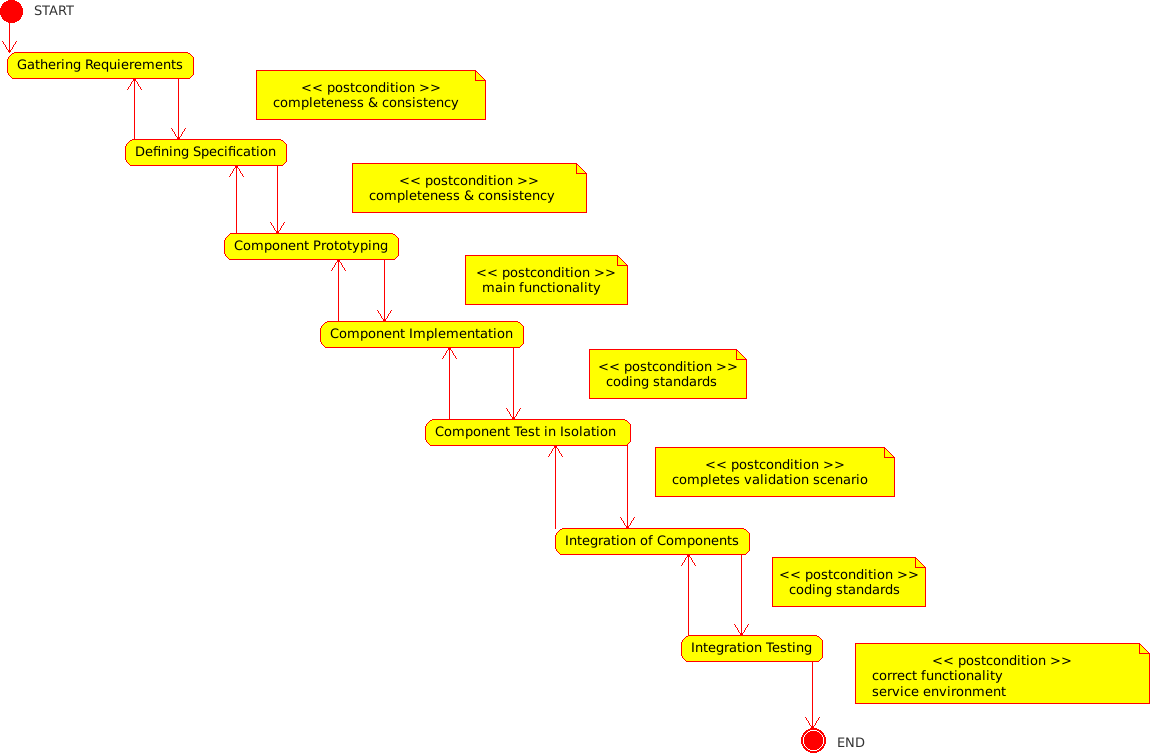
\includegraphics[width=4in]{img/stepwise_validation_process.png}
\end{frame}

\section{Demo Application}
\begin{frame}
  \frametitle{Demo Application}
  \framesubtitle{Sequence Diagram}
  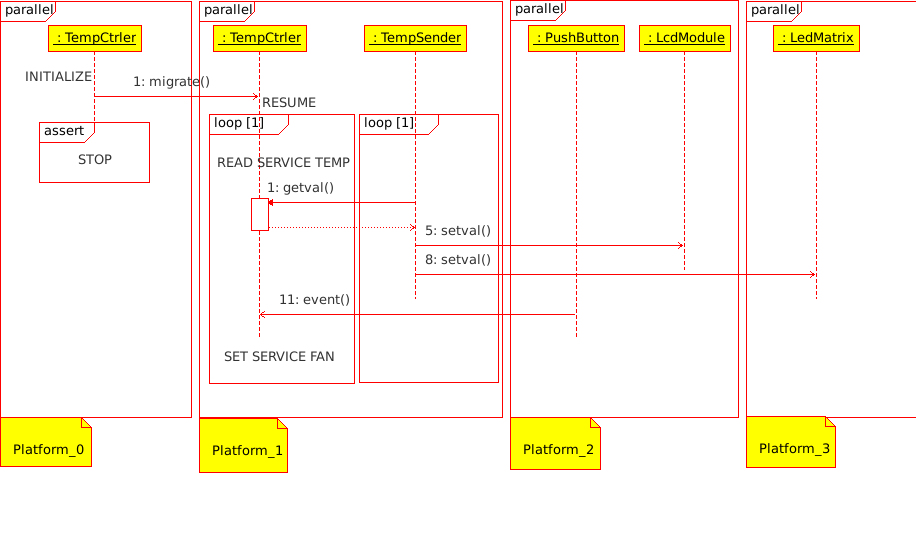
\includegraphics[width=4in]{img/sequence-diagram-demoapp.png}
\end{frame}


% End of document
\end{document}
